\documentclass[14pt,a4paper,report]{report}
\usepackage[a4paper, mag=1000, left=2.5cm, right=1cm, top=2cm, bottom=2cm, headsep=0.7cm, footskip=1cm]{geometry}
\usepackage[utf8]{inputenc}
\usepackage[english,russian]{babel}
\usepackage{indentfirst}
\usepackage[dvipsnames]{xcolor}
\usepackage[colorlinks]{hyperref}
\usepackage{listings} 
\usepackage{fancyhdr}
\usepackage{caption}
\usepackage{amsmath}
\usepackage{latexsym}
\usepackage{graphicx}
\usepackage{amsmath}
\usepackage{booktabs}
\usepackage{array}
\hypersetup{
	colorlinks = true,
	linkcolor  = black
}

\usepackage{titlesec}
\titleformat{\chapter}
{\Large\bfseries} % format
{}                % label
{0pt}             % sep
{\huge}           % before-code


\DeclareCaptionFont{white}{\color{white}} 

% Listing description
\usepackage{listings} 
\DeclareCaptionFormat{listing}{\colorbox{gray}{\parbox{\textwidth}{#1#2#3}}}
\captionsetup[lstlisting]{format=listing,labelfont=white,textfont=white}
\lstset{ 
	% Listing settings
	inputencoding = utf8,			
	extendedchars = \true, 
	keepspaces = true, 			  	 % Поддержка кириллицы и пробелов в комментариях
	language = Matlab,            	 	 % Язык программирования (для подсветки)
	basicstyle = \small\sffamily, 	 % Размер и начертание шрифта для подсветки кода
	numbers = left,               	 % Где поставить нумерацию строк (слева\справа)
	numberstyle = \tiny,          	 % Размер шрифта для номеров строк
	stepnumber = 1,               	 % Размер шага между двумя номерами строк
	numbersep = 5pt,              	 % Как далеко отстоят номера строк от подсвечиваемого кода
	backgroundcolor = \color{white}, % Цвет фона подсветки - используем \usepackage{color}
	showspaces = false,           	 % Показывать или нет пробелы специальными отступами
	showstringspaces = false,    	 % Показывать или нет пробелы в строках
	showtabs = false,           	 % Показывать или нет табуляцию в строках
	frame = single,              	 % Рисовать рамку вокруг кода
	tabsize = 2,                  	 % Размер табуляции по умолчанию равен 2 пробелам
	captionpos = t,             	 % Позиция заголовка вверху [t] или внизу [b] 
	breaklines = true,           	 % Автоматически переносить строки (да\нет)
	breakatwhitespace = false,   	 % Переносить строки только если есть пробел
	escapeinside = {\%*}{*)}      	 % Если нужно добавить комментарии в коде
}

\begin{document}

\def\contentsname{Содержание}

% Titlepage
\begin{titlepage}
	\begin{center}
		\textsc{Санкт-Петербургский Политехнический 
			Университет Петра Великого\\[5mm]
			Кафедра компьютерных систем и программных технологий}
		
		\vfill
		
		\textbf{Отчёт по лабораторной работе №4\\[3mm]
			Курс: «Методы оптимизации и принятия решений»\\[3mm]
			Тема: «Анализ GERT-сети»\\[35mm]
			}
	\end{center}
	
	\hfill
	\begin{minipage}{.5\textwidth}
		Выполнил студент:\\[2mm] 
		Бояркин Никита Сергеевич\\
		Группа: 13541/3\\[5mm]
		
		Проверил:\\[2mm] 
		Сиднев Александр Георгиевич
	\end{minipage}
	\vfill
	\begin{center}
		Санкт-Петербург\\ \the\year\ г.
	\end{center}
\end{titlepage}

% Contents
\tableofcontents
\clearpage

\chapter{Лабораторная работа №4}

\section{Индивидуальное задание}

\subsubsection{Задача 25}

\begin{figure}[h!]
	\centering
	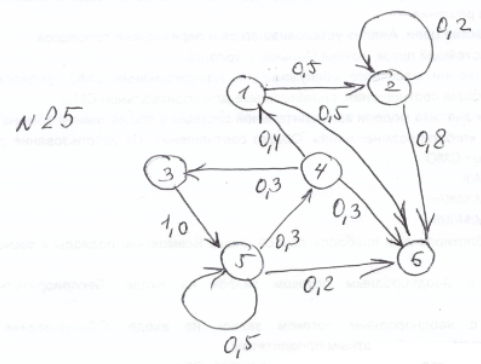
\includegraphics[scale = 0.95]{images/0.png}
	\caption{Исходный граф системы}
	\label{image:0}
\end{figure}

Каждой дуге ($ij$) поставлены в соответствие следующие данные:

\begin{itemize}
	\item Закон распределения времени выполнения работы. Будем считать его нормальным.
	\item Параметры закона распределения (математическое ожидание $M$ и дисперсия $D$).
	\item Вероятность $P_{ij}$ выполнения работы, показанная на графе.
\end{itemize}

Необходимо найти:

\begin{itemize}
	\item Вероятность выхода в завершающий узел графа (для всех вариантов узел 6).
	\item Математическое ожидание.
	\item Дисперсию времени выхода процесса в завершающий узел графа.
\end{itemize}

В отчете перечислить все петли всех порядков, обнаруженные на графе, выписать уравнение Мейсона, получить решение для $W_E(s)$ и найти требуемые параметры.

\subsubsection{Дополнительное задание}

Решить задачу используя методику анализа потокового графа, основанную на обработке матрицы передач (Branch Transmittance Matrix).

\clearpage

\section{Ход работы}

\subsection{Построение замкнутой GERT-сети}

Чтобы определить эквивалентную W-функцию для анализируемой GERT-сети, необходимо замкнуть сеть дугой, исходящей из узла 6 в узел 1:

\begin{figure}[h!]
	\centering
	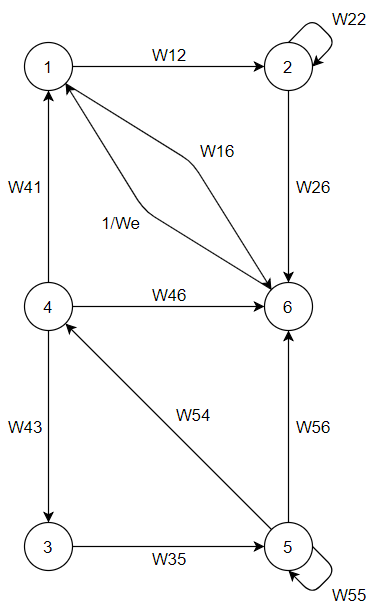
\includegraphics[scale = 0.55]{images/1.png}
	\caption{Замкнутая GERT-сеть}
	\label{image:1}
\end{figure}

\subsection{Построение W-функции}

Найдем W-функции для дуг GERT-сети:

\begin{table}[h!]
	\centering
	\bgroup
	\def\arraystretch{1}
	\begin{tabular}{ | m{1.4cm} | m{1.4cm} | m{1.9cm} | m{2.4cm} | m{2.0cm} | m{2.4cm} | }
		\hline
		Начало & Конец & Вероятность & Мат. ожидание & Дисперсия & W-функция \\ \hline
		1 & 2 & 0.5 & 10 & 4 & $0.5\cdot e^{10t+8t^2}$ \\ \hline
		1 & 6 & 0.5 & 23 & 25 & $0.5\cdot e^{23t+312.5t^2}$ \\ \hline
		2 & 2 & 0.2 & 13 & 16 & $0.2\cdot e^{13t+128t^2}$ \\ \hline
		2 & 6 & 0.8 & 11 & 16 & $0.8\cdot e^{11t+128t^2}$ \\ \hline
		3 & 5 & 1 & 10 & 9 & $1\cdot e^{10t+40.5t^2}$ \\ \hline
		4 & 1 & 0.4 & 37 & 16 & $0.4\cdot e^{37t+128t^2}$ \\ \hline
		4 & 3 & 0.3 & 12 & 16 & $0.3\cdot e^{12t+128t^2}$ \\ \hline
		4 & 6 & 0.3 & 12 & 49 & $0.3\cdot e^{12t+1200.5t^2}$ \\ \hline
		5 & 4 & 0.3 & 15 & 25 & $0.3\cdot e^{15t+312.5t^2}$ \\ \hline
		5 & 5 & 0.5 & 19 & 4 & $0.5\cdot e^{19t+8t^2}$ \\ \hline
		5 & 6 & 0.2 & 42 & 9 & $0.2\cdot e^{42t+40.5t^2}$ \\
		\hline
	\end{tabular}
	\egroup
\end{table}

\subsection{Построение уравнения Мейсона}

Найдем все петли первого порядка:

$W_{12}\cdot W_{26}\cdot \frac{1}{W_E}$

$W_{16}\cdot \frac{1}{W_E}$

$W_{35}\cdot W_{54}\cdot W_{43}$

$W_{22}$

$W_{55}$\\

Найдем все петли второго порядка:

$W_{16}\cdot W_{22}\cdot \frac{1}{W_E}$

$W_{16}\cdot W_{35}\cdot W_{54}\cdot W_{43}\cdot \frac{1}{W_E}$

$W_{16}\cdot W_{55}\cdot \frac{1}{W_E}$

$W_{12}\cdot W_{26}\cdot W_{55}\cdot \frac{1}{W_E}$ 

$W_{12}\cdot W_{26}\cdot W_{35}\cdot W_{54}\cdot W_{43}\cdot \frac{1}{W_E}$

$W_{22}\cdot W_{55}$

$W_{22}\cdot W_{35}\cdot W_{54} \cdot W_{43}$\\

Найдем все петли третьего порядка:

$W_{16}\cdot W_{22}\cdot W_{35}\cdot W_{54}\cdot W_{43}\cdot \frac{1}{W_E}$

$W_{16}\cdot W_{22}\cdot W_{55}\cdot \frac{1}{W_E}$\\

Таким образом уравнение Мейсона будет иметь следующий вид:

$H=1-(W_{12}W_{26}\frac{1}{W_E}+W_{16}\frac{1}{W_E}+W_{35}W_{54}W_{43}+W_{22}+W_{55})+(W_{16}W_{22}\frac{1}{W_E}+W_{16}W_{35}W_{54}W_{43}\frac{1}{W_E}+W_{16}W_{55}\frac{1}{W_E}+W_{12}W_{26}W_{55}\frac{1}{W_E}+W_{12}W_{26}W_{35}W_{54}W_{43}\frac{1}{W_E}+W_{22}W_{55}+W_{22}W_{35}W_{54} W_{43})-(W_{16}W_{22}W_{35}W_{54}W_{43}\frac{1}{W_E}+W_{16}W_{22}W_{55}\frac{1}{W_E})$\\

В результате эквивалентная W-функция равняется:

$W_E(s)=\frac{W_{12}W_{26}+W_{16}-W_{16}W_{22}-W_{16}W_{35}W_{54}W_{43}-W_{16}W_{55}-W_{12}W_{26}W_{55}-W_{12}W_{26}W_{35}W_{54}W_{43}+W_{16}W_{22}W_{35}W_{54}W_{43}+W_{16}W_{22}W_{55}}{1-W_{35}W_{54}W_{43}-W_{22}-W_{55}+W_{22}W_{55}+W_{22}W_{35}W_{54} W_{43}}$\\

\subsection{Рассчет статистических значений}

Расчет математического ожидания ($\mu_{1E}$) и дисперсии ($\sigma_E$) производится по следующим образом:

$W_E(s)=p_E\cdot M_E(s), p_E=W_E(0)\Longrightarrow M_E(s)=\frac{W_E(s)}{W_E(0)}$

$\mu_{1E}=\frac{d M_E(s)}{ds}|s=0$

$\mu_{2E}=\frac{d^2 M_E(s)}{ds^2}|s=0$

$\sigma_E=\mu_{2E}-\mu_{1E}^2$\\

Разработаем скрипт для расчета статистических значений в среде MATLAB:

\lstinputlisting{listings/l1.m}

Результат вычисления статистических значений:

\lstinputlisting{listings/l1.log}

\subsection{Дополнительное задание}

Для данного метода W-функция $W_e$ расчитывается по формуле:

$M_{1n}=\frac{1}{w_{n1}}=-\frac{\frac{\delta det(\tilde{A})}{\delta w_{n1}}}{det(\tilde{A}|_{w_{n1}=0})}$, где\\

$n=6,\tilde{A}=I_n-\tilde{Q}^T,A=I-Q^T,q_{ij}(s)=p_{ij}m_{ij}(s)$

Разработаем скрипт для расчета статистических значений при помощи анализа потокового графа в среде MATLAB:

\lstinputlisting{listings/l2.m}

Результат вычисления статистических значений:

\lstinputlisting{listings/l2.log}

Результаты идентичны предыдущему решению, за исключением $W_e(0)$, что объясняется результирующей функцией взятой с обратным знаком.

\section{Вывод}

В ходе данной лабораторной работы были получены навыки работы с вероятностными графами и их обработка с помощью методики GERT. При заданных значениях вероятности, мат. ожидания и дисперсии для каждой дуги исходного графа достаточно легко расчитываются W-функции, которые необходимы для построения формулы Мейсона. После этого из формулы Мейсона по формулам математической статистики достаточно легко расчитывается результирующее мат. ожидание и дисперсия.

Решение путем анализа потокового графа показало аналогичные результаты, что подтверждает корректность решения. Однако, метод анализа потокового графа выполняется заметно медленнее, даже на небольшом графе.

\end{document}